\subsection{Artifacts}

Finalmente, analizaremos los llamados ``artifacts'', los cuales podr\'ian ser definidos como alteraciones anormales de los videos. Sin embargo, generar estos artifacts puede llegar a ser d\'ificil dado que no solo requiere de varias combinaciones de pruebas y videos, sino tambi\'en agudizar la vista para poder encontrarlos. Ante esto, y como primera estrategia para generarlos, tomamos el video \textbf{camerachanges.mp4}, el cual posee una gran cantidad de cambios de c\'amara, y decidimos alentarlo 3 veces consecutivas (interpolando 1 frame entre cada par de frames) con cada uno de los 3 m\'etodos. En consecuencia, los videos generados tendr\'an 3 veces m\'as frames que el original.

Luego de realizar las pruebas, analizamos a ojo los 3 videos (1 por m\'etodo) altamente alentados y detectamos lo siguiente para cada m\'etodo:

\begin{enumerate}
\item M\'etodo m\'as cercano: al alentar varias veces el video con este m\'etodo, el resultado es equivalente a un slide de im\'agenes que se pasa lentamente, esto es, muchos frames iguales por segundo. Este efecto era esperable dado que este m\'etodo genera un nuevo frame id\'entico al frame m\'as cercano, por lo cual ejecutarlo consecutivamente solo generar\'a copias de frames entre frames ya existentes. Es por eso que el video en este caso no presenta ninguna alteraci\'on en los frames que sea visible a ojo dado que los nuevos frames no son distintos a los ya existentes en el video original.
\item M\'etodo interpolaci\'on lineal: en este m\'etodo pudimos detectar un efecto al que vamos a llamar ``ghosting'', y que lo vamos a definir como el frame generado por la superposici\'on del frame anterior y el siguiente del que presenta este efecto. Este efecto sucede debido a que al ocurrir cambios bruscos entre frames, interpolaci\'on lineal intentar\'a generar un frame intermedio entre ambos. El efecto se puede apreciar en la figura 1.

\begin{figure}[h!]
  \centering
    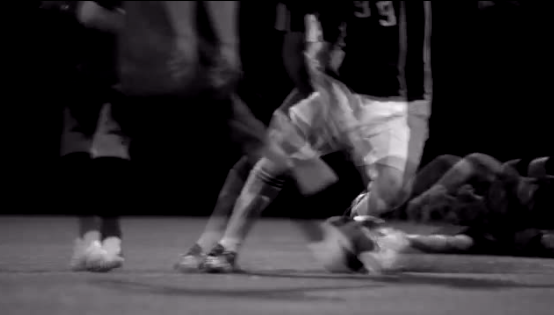
\includegraphics[width=0.5\textwidth]{img/artifact_lineal.png}
  	\caption{Ghosting, el artifact de interpolaci\'on lineal.}
\end{figure}

\begin{figure}[h!]
  \centering
    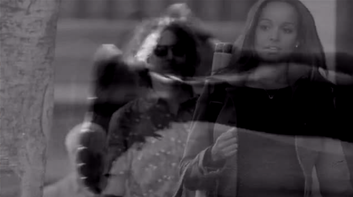
\includegraphics[width=0.5\textwidth]{img/ghosting_splines_1.png}
  	\caption{Ghosting en splines para el cambio de c\'amara.}
\end{figure}

\begin{figure}[h!]
  \centering
    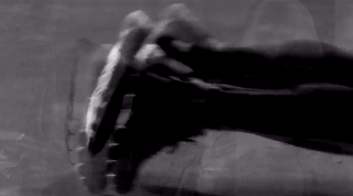
\includegraphics[width=0.5\textwidth]{img/ghosting_negative.png}
  	\caption{Frame en negativo con superposici\'on con otro frame en splines.}
\end{figure}

\item M\'etodo splines: para el video generado por este momento, detectamos que se genera el mismo efecto de ghosting que en con interpolaci\'on lineal, dado que tambi\'en es un tipo de interpolaci\'on. Sin embargo, hemos detectado una alteraci\'on extra. Esta alteraci\'on produce un efecto interesante, por el cual luego de un efecto de ghosting en los frames de la transici\'on de un cambio de c\'amara, el frame anterior al cambio de c\'amara vuelve a aparecer en negativo en superposici\'on con los frames luego del cambio de c\'amara. Para apreciar este efecto, se pueden observar las figuras 2 y 3.

\end{enumerate}

Adem\'as, realizamos otros experimentos interpolando varios frames entre cada par de frames del video original, pero no logramos obtener alg\'un efecto distinto a los ya mencionados. Incluso experimentamos con videos sin cambios de c\'amara, pero sin nuevos resultados.
